\documentclass[11pt]{article}
  
%%% LATEX COMMON Packages 

\usepackage[bookmarks,colorlinks,breaklinks]{hyperref}  % PDF hyperlinks, with coloured links
\hypersetup{linkcolor=blue,citecolor=blue,filecolor=blue,urlcolor=blue} % all blue links
\usepackage{amsmath,amsfonts,amsthm,amssymb,environ,xstring}
\usepackage{dsfont}
\usepackage{fullpage}
\usepackage{mdframed}
\usepackage{tikz}
\usetikzlibrary{automata, positioning, arrows}
\tikzset{
    ->, % makes the edges directed
    >=stealth, % makes the arrow heads bold
    node distance=3cm, % specifies the minimum distance between two nodes. Change if necessary.
    every state/.style={thick}, % sets the properties for each ’state’ node
    initial text=$ $, % sets the text that appears on the start arrow
}
\usepackage{graphicx}
\newcommand{\ignore}[1]{}
\newcommand \kw[1]{\textbf{#1}}
\newenvironment{answer}{
\vspace{.5cm}
\begin{mdframed}[]
    \kw{Answer} 
}
{
\end{mdframed}
\pagebreak
}

\title{\bf{CS 181 Homework 3}}
\author{ Einar Balan }
\date{}
\begin{document}
\maketitle



\begin{enumerate}
%\item Show that for any NFA $N$, there exists a NFA $N'$ that is equivalent to $N$ (i.e., computes the same function as $N$) such that every state has at most one outgoing edge for each of labels $0$ or $1$. That is, in the diagram of $N'$, no state has two outgoing edges that are both labeled $0$ or $1$. [.5 point]

%You must solve this problem without using the theorem from class that every NFA can be converted to a DFA and without increasing the number of states exponentially.

\item As we mentioned in class the critical part of KMP string matching algorithm is the following: Given a pattern $p \in \{0,1\}^*$, we have to design a DFA that accepts only those strings that contain $p$. Let us explore this idea for a bit.

Suppose the pattern $p$ is $0110$, can you design a DFA that only accepts strings that contain this pattern? 

\begin{answer}
    \begin{center}
        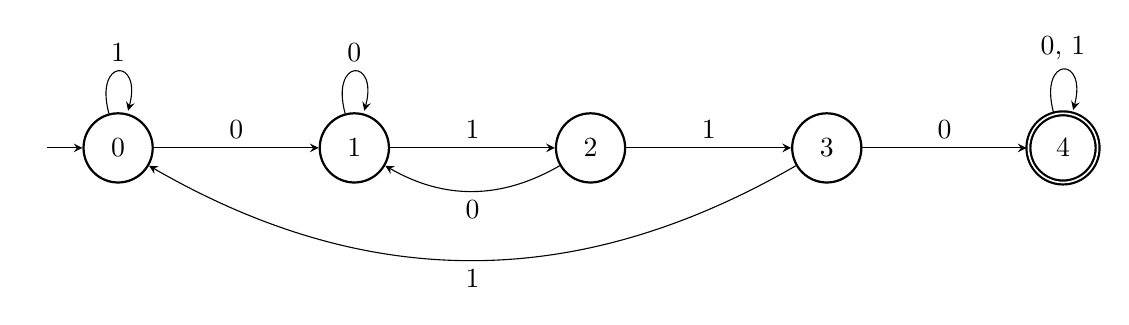
\begin{tikzpicture}
            \node[state, initial] (q0) {0};
            \node[state, right of=q0] (q1) {1};
            \node[state, right of=q1] (q2) {2};
            \node[state, right of=q2] (q3) {3};
            \node[state, accepting, right of=q3] (q4) {4};

            \draw   (q0) edge[above] node{0} (q1)
                    (q0) edge[loop above] node{1} (q0)
                    (q1) edge[loop above] node{0} (q1)
                    (q1) edge[above] node{1} (q2)
                    (q2) edge[bend left, below] node{0} (q1)
                    (q2) edge[above] node{1} (q3)
                    (q3) edge[bend left, below] node{1} (q0)
                    (q3) edge[above] node{0} (q4)
                    (q4) edge[loop above] node{0, 1} (q4);
        \end{tikzpicture}
    \end{center}

    The DFA above works by only progressing to the next state when the correct bit is seen. If it is not seen, then the state is reset to the state which would have been progressed to if the bit was read frrom the initial state. Once we encounter $p$, we enter a persistent accepting state.

\end{answer}


\item Converting a regular expression to an NFA. In class, we saw a procedure to build a NFA for every regular expression r. Let us understand the `size' of the NFA created by this procedure as a function of the length of the regular expression r. Here, length of the regular expression refers to the number of characters in the regular expression. 

Suppose the regular expression $r$ had length $m$. How many states would be present in the final NFA built by the procedure in class as a function of $m$ (use big-Oh notation and avoid computing constants)? Explain your reasoning in a few sentences [.5 points]

Here, by size of a regex you can take it to mean the length of the string that corresponds to the regex. For instance, the regex $(01)^*$ would have size 5. Alternately, more intuitively, you can take size to mean the number of recursive subpieces and operations that you'd see within the regular expression. Any way you interpret the size, the answer should be same up to big-Oh notation. 

Do not worry about figuring out the edge-cases and/or the exact constants.

[Hint: Look at each of the steps in the compound case, and see how the number of states can increase.]

\begin{answer}
    $O(m)$ states.

    \vspace{.5cm}

    Considering base cases:
    \begin{itemize}
        \item ``0'' regex has an NFA with 2 states
        \item ``1'' regex has an NFA with 2 states
    \end{itemize}

    Considering each compound case:
    \begin{itemize}
        \item concatenation simply adds epsilon transitions from accepting states of the first NFA to the initial state of the second, so performing $c$ concatenations in the regex will add no states beyond the base cases 
        \item union can be computed by adding a new inital state with epsilon transitions to both original initial states, so if there are $u$ unions in the regex this translates to adding $u$ states in the NFA
        \item kleen* is computed by adding a new inital state and epsilon transitions, so if there are $k$ kleen* operations in the regex this translates to adding $k$ states in the NFA
    \end{itemize} 

    So if there are $n$ 0s or 1s in the regex, we will have at most $2n$ states in the NFA representing them. We know that each of $n, c, u, k < m \therefore O(2n + 0c + u + k) = O(m)$ states in the NFA.
\end{answer}

\item Design a regular expression for the following language: 
$$L = \{x: \text{ every $1$ in $x$ is followed by at least two zeroes }\}.$$
For instance, $010010000,1000,0010010000$ are in the language but $10101, 011001000$ are not.You don't have to prove your expression works but write a few sentences describing why your expression could/does work. [.75 point]

\begin{answer}
    $r = (0 | 100)^*$

    \vspace{.5cm}

    At every point, we only want to accept a string that is either a 0 or a 1 followed by two 0s. We use the union operation to capture 0 or 100 and we use kleene* to extend this logic to every point in the string.
\end{answer}

\item Show that the following functions/languages are not regular: 
\begin{enumerate}
\item $L = \{x: x = 0^m 1^{3m}\}$. For instance, $0111, 00111111$ would be in $L$, but $0100, 0011$ would not be elements of $L$. [.75 points]

%[Hint: It might be easier to \emph{pump down}, i.e., the case $i=0$ in the pumping lemma for the problem.]
\item $F:\{0,1\}^* \rightarrow \{0,1\}$ defined by $F(x) = 1$ if and only if $x = 1^{i^3}$ for some $i > 0$. [.75 points]
\item $UNEQUAL = \{0^m 1 0^n: m \neq n\}$. [.75 points]

% [Hint: This one is a bit tricky (but remember the relaxed grading scheme). You can try to directly show the language is not regular by using the pumping lemma by a careful choice of $m,n$. Think what choice of $m,n$ would allow that repeating a piece of the first block of $0$'s can match the length of the second block of $0$'s? (You'll have to look at factorials ...). 

% An alternate approach is to use closure properties of regular languages: recall the following corollary of what we showed in class if $L, L'$ are regular then $L \setminus L' = L \cap (\overline{L'})$ is also regular (because $\overline{L'}$ is regular; and the intersection of two regular languages ir regular). Can you find a regular language $L$ such that $L \setminus UNEQUAL$ can be shown to be not regular by pumping lemma much more easily? ]
\end{enumerate}

 Your proofs should be at the similar level of detail as the examples from lecture 11; that is, write down the different steps as we did in class.

 \begin{answer}
    \begin{enumerate}
        \item Suppose $L$ was regular. Then there must exist $p$ such that PL holds. Consider $x = 0^p1^{3p}$, which is in the language and has length greater than $p$. If we split $x$ into $a, b, \text{and } c$ subcomponents such that length($ab$) $\le p$, then $abbc$ is not in the language. This is because we know that the split between a and b must lie within the section of 0's due to the length restriction. So no matter what, pumping b will result in changing the number of 0's while leaving the number of 1's constant and the number of 1's will no longer be 3 times the number of 0's. This is a contradiction, so L must not be regular.
        \item Suppose $F$ was regular. Then there must exist $p$ such that PL holds. Consider $x = 1^{p^3}$, which is in the language and has length greater than $p$. If we split $x$ into $a, b, \text{and } c$ subcomponents such that length($ab$) $\le p$, then $ab^0c$ is not in the language. We know that $0 < \text{length}(b) \le p$ so the length $l$ of $ab^0c$ is $p^3 - p \le l < p^3$. The previous cube is $(p - 1)^3 = p^3-3p^2+3p-1$ which is less than the range of lengths possible for $ab^0c$, therefore it must not be in the language. This is a contradiction, so L must not be regular. 
        \item Consider $L = \{x: \text{starting and ending bits are the same}\}$. We know $L$ is regular because it is computed by the regex $r$ = ((0(0$|$1)$^*$0) $|$ (1(0$|$1)$^*$)1). Suppose that $UNEQUAL$ is regular as well. Then there must exist $p$ such that PL holds for $L \setminus UNEQUAL$ (by closure properties). Also consider $x = 0^p10^p$, which is in $L \setminus UNEQUAL$. If we split x into $a, b, \text{and } c$ subcomponents such that length($ab$) $\le p$, then $abbc$ is not in the language. This is because we know that the split between a and b must lie within the first section of 0's due to the length restriction, so no matter what pumping b will only change the number of 0's in the first section, causing the string to be in $UNEQUAL$ and therefore not in $L \setminus UNEQUAL$. This is a contradiction, so $L \setminus UNEQUAL$ must not be regular. We showed $L$ was regular, so it must be that $UNEQUAL$ is not regular.
    \end{enumerate}
\end{answer}

\end{enumerate}



{\bf Additional practice problems - Not to be graded}

\begin{enumerate}
\item (COMMENTED OUT) Show that if a language $L$ is regular, then so is $Reverse(L) = \{x: Reverse(x) \in L\}$. 

\item Design a regular expression for the following languages: 
\begin{itemize}
\item $L = \{x: \text{ third bit from end of $x$ is a 1}\}$.
% \begin{itemize}
%     \item $(0|1)^*1(0|1)(0|1)$
% \end{itemize}
\item $L = \{x: \text{ number of $1$'s in $x$ is divisible by $5$}\}$.
% \begin{itemize}
%     \item $((0)^*1(0)^*1(0)^*1(0)^*1(0)^*1(0)^*)^*$
% \end{itemize}
\item $L = \{x: \text{ $x$ has an odd number of $1$'s}\}$. 
% \begin{itemize}
%     \item 
% \end{itemize}
\item $L = \{x: \text{ $x$ has at least three $1$'s}\}$.
% \begin{itemize}
%     \item $((0)^*1(0)^*1(0)^*1(0)^*)(0|1)^*$
% \end{itemize}
\item L = All strings except the empty string.
% \begin{itemize}
%     \item $(0|1)(0|1)*$
% \end{itemize}
\item $L = \{x: \text{ $x$ has an even number of $0$'s or contains exactly two $1$'s}\}$.
\end{itemize}

\item Continuing problem (2) above:
\begin{enumerate}
\item[3a] How many transitions/edges are present in the final NFA built by the procdure in class as a function of $m$ (use big-Oh notation and avoid computing constants)?

[Hint: Look at each of the steps in the compund case, and see how the number of edges added changes.] 

\item[3b] (Advanced) Do you see a way to modify the procedure to only add at most $O(m)$ transitions in the NFA? Such an NFA is what gets used in grep and other regex matching tools.

[Hint: The most expensive step in terms of number of edges added is the compound case corresponding to the (*) operation. What happens if you maintain the invariant that all the NFAs you build only have one accept state?Can we maintain this invariant?]
\end{enumerate}

\item Show that the following languages are not regular.
\begin{enumerate}
    \item $L = \{ 0^{|w|} \circ w: w \in \{0, 1\}^*\}$
    \item $L = \{ ww: w \in \{0, 1\}^*\}$
\end{enumerate}

\end{enumerate}


\end{document}
